%%%%%%%%%%%%%%%%%%%%%%%%%%%%%%%%%%%%%%%%%
% Journal Article
% LaTeX Template
% Version 1.4 (15/5/16)
%
% This template has been downloaded from:
% http://www.LaTeXTemplates.com
%
% Original author:
% Frits Wenneker (http://www.howtotex.com) with extensive modifications by
% Vel (vel@LaTeXTemplates.com)
%
% License:
% CC BY-NC-SA 3.0 (http://creativecommons.org/licenses/by-nc-sa/3.0/)
%
%%%%%%%%%%%%%%%%%%%%%%%%%%%%%%%%%%%%%%%%%

%----------------------------------------------------------------------------------------
%	PACKAGES AND OTHER DOCUMENT CONFIGURATIONS
%----------------------------------------------------------------------------------------

%\documentclass{article}
\documentclass[oneside,twocolumn]{article}

\usepackage{blindtext} % Package to generate dummy text throughout this template 
\usepackage{multicol}
\usepackage[sc]{mathpazo} % Use the Palatino font
\usepackage[T1]{fontenc} % Use 8-bit encoding that has 256 glyphs
\linespread{1.05} % Line spacing - Palatino needs more space between lines
\usepackage{microtype} % Slightly tweak font spacing for aesthetics

\usepackage[english]{babel} % Language hyphenation and typographical rules

\usepackage[hmarginratio=1:1,top=32mm,columnsep=20pt]{geometry} % Document margins
\usepackage[hang, small,labelfont=bf,up,textfont=it,up]{caption} % Custom captions under/above floats in tables or figures
\usepackage{booktabs} % Horizontal rules in tables

\usepackage{lettrine} % The lettrine is the first enlarged letter at the beginning of the text

\usepackage{enumitem} % Customized lists
\setlist[itemize]{noitemsep} % Make itemize lists more compact

\usepackage{abstract} % Allows abstract customization
\renewcommand{\abstractnamefont}{\normalfont\bfseries} % Set the "Abstract" text to bold
\renewcommand{\abstracttextfont}{\normalfont\small\itshape} % Set the abstract itself to small italic text

\usepackage{titlesec} % Allows customization of titles
\renewcommand\thesection{\Roman{section}} % Roman numerals for the sections
\renewcommand\thesubsection{\roman{subsection}} % roman numerals for subsections
\titleformat{\section}[block]{\large\scshape\centering}{\thesection.}{1em}{} % Change the look of the section titles
\titleformat{\subsection}[block]{\large}{\thesubsection.}{1em}{} % Change the look of the section titles

\usepackage{fancyhdr} % Headers and footers
\pagestyle{fancy} % All pages have headers and footers
\fancyhead{} % Blank out the default header
\fancyfoot{} % Blank out the default footer
%\fancyhead[C]{Running title $\bullet$ May 2016 $\bullet$ Vol. XXI, No. 1} % Custom header text
\fancyfoot[RO,LE]{\thepage} % Custom footer text

\usepackage{titling} % Customizing the title section

\usepackage{hyperref} % For hyperlinks in the PDF

\usepackage{listings}
\usepackage{algorithm2e}
\usepackage{graphicx}
\usepackage[dvipsnames]{xcolor}
\definecolor{codegreen}{rgb}{0,0.6,0}
\definecolor{codegray}{rgb}{0.5,0.5,0.5}
\definecolor{codepurple}{rgb}{0.58,0,0.82}
\definecolor{backcolour}{rgb}{1,1,1}
\lstdefinestyle{mystyle}{
    backgroundcolor=\color{backcolour},   
    commentstyle=\color{codegreen},
    keywordstyle=\color{magenta},
    numberstyle=\tiny\color{codegray},
    stringstyle=\color{codepurple},
    basicstyle=\ttfamily\footnotesize,
    breakatwhitespace=false,         
    breaklines=true,                 
    captionpos=b,                    
    keepspaces=true,                 
    numbers=left,                    
    numbersep=5pt,                  
    showspaces=false,                
    showstringspaces=false,
    showtabs=false,                  
    tabsize=2
}
\renewcommand{\lstlistingname}{Código}% Listing -> Algorithm
\lstset{style=mystyle}

%----------------------------------------------------------------------------------------
%	TITLE SECTION
%----------------------------------------------------------------------------------------

\setlength{\droptitle}{-4\baselineskip} % Move the title up

\pretitle{\begin{center}\Huge\bfseries} % Article title formatting
\posttitle{\end{center}} % Article title closing formatting
\title{Wavefront Propagation} % Article title
\author{%
\textsc{Luis Alberto Ballado Aradias} \\%\thanks{A thank you or further information} \\[1ex] % Your name
\normalsize Cinvestav Unidad Tamaulipas \\ % Your institution
\normalsize \href{mailto:luis.ballado@cinvestav.mx}{luis.ballado@cinvestav.mx} % Your email address
%\and % Uncomment if 2 authors are required, duplicate these 4 lines if more
%\textsc{Jane Smith}\thanks{Corresponding author} \\[1ex] % Second author's name
%\normalsize University of Utah \\ % Second author's institution
%\normalsize \href{mailto:jane@smith.com}{jane@smith.com} % Second author's email address
}
\date{\today} % Leave empty to omit a date
\renewcommand{\maketitlehookd}{%
\begin{abstract}
\noindent The task of building a map of an unknown environment and concurrently using that map to navigate is a central problem in mobile robotics research. This document trys to replicate one of the knows algorithm (wavefront expansion) to explore a map using plan C code in the first phase and parallelizate it to perform its calculations trying to reduce the total computation time. Parallel wavefront expansion can significantly improve the computational performance and speed of the algorithm, particularly when processing large environments or complex obstacles. By utilizing multiple processing units, the algorithm should process the environment, reducing the total computation time. However, parallel software also has some limitations, such as increased complexity in implementation and increased communication overhead between processing units. It is important to consider these limitations.

\end{abstract}
}

%----------------------------------------------------------------------------------------

%One of the major applications of mobile robots is to create models of the environment they traverse using sensor data; this process is known as mapping. Military applications of this technology are obvious. Visualize a robot that somehow enters a vacant building in hostile territory. For example, it could be thrown through an open window, crawl through drain pipes, or climb up the side of the building. Once inside, the robot can traverse the hallways and create a map showing doors, hall crossing, stairways, and other features.

%The most commonly used approaches to mapping are termed "grid based or metric mapping and topological mapping".
%Metric or quantitative maps, as the name implies, are based on measurements of the space they map. An indoor metric map may include the lengths of wall sections, door-opening widths, hallways widths, distances to intersections, and so forth. A typical metric navigation instruction might be "Move 45 meters in north direction, then turn 30º clockwise and move another 65 meters.
%Path planning in metrically mapped spaces usually includes the designation of a number of way points at specific (x,y) locations, connected by straight-line segments. Paths can then be selected on the basis of some optimization criterion.
%A widely used method of generationg a metric map is to cover the environment to be mapped with an evently spaced grid. Each cell in the grid is then filled with one or more values that represent the presence or absence of an obstacle (which could be another robot or a human).Grid-based mapping was first proposed in the 1980's  by Elfes

\begin{document}

% Print the title
\maketitle

%----------------------------------------------------------------------------------------
%	ARTICLE CONTENTS
%----------------------------------------------------------------------------------------


    
\section{Introduction}

\lettrine[nindent=0em,lines=3]{W} avefront expansion is a popular path planning algorithm used in mobile robotics for determining the optimal path for a robot to move from its starting position to its goal while avoiding obstacles. The algorithm starts with the goal position and creates a wavefront that expands outward, considering the surrounding environment and updating the cost of reaching each cell. The final path is determined by selecting the lowest cost path from the starting position to the goal.\\

Beginning with mid-1960s, the path planning has attracted interests from a lot of scholars. The path planning problem can be described in the following: given a robot and its working environment, the mobile robots searches for an optimal or suboptimal path from the initial state to the target state according to a certain performance criteria. Good path planning technology of mobile robot can not only save a lot of time, but also reduce the wear and capital investment of mobile robot.\\

Wavefront expansion is well-suited for real-time applications, as it can be executed efficiently in terms of computation time. The algorithm can handle complex environments with many obstacles and can produce an optimal path in a relatively short amount of time. Additionally, the algorithm can be modified to incorporate additional objectives, such as time constraints or energy consumption, by incorporating different cost functions.\\

One of the key benefits of wavefront expansion is its simplicity, which makes it easy to understand and implement. The algorithm is also highly flexible, as it can be adapted to various types of robots and environments, from ground robots to aerial robots, and from indoor to outdoor environments. \\

However, wavefront expansion has some limitations that need to be considered. For example, the algorithm does not consider the dynamics of the robot or the motion constraints of the environment. As a result, the final path produced by the algorithm may not be feasible for the robot to follow.

%------------------------------------------------

\newpage
\onecolumn
\section{Serial Algorithm}

The typical wavefront expansion algorithm uses the implementation of an adjacency list representation of graphs, storing the lists of adjacent nodes and the queue of nodes needed for BFS traversal.\\

At this first phase I am not using the BFS algorithm (because of my data-structure issues), not discarding also develop the bfs version of the algorithm and compare the results applying the parallelism techniques.\\

The serial main program consists of the invocation of five functions:

\begin{itemize}
\item \textbf{map\_init:} Initialize the map
\item \textbf{propagate\_wavefront:} main function of the algorithm in charge of propagating and coordinating the exploration of new nodes to visit
\item \textbf{clear\_map:} just crear the map for another experiments
\item \textbf{explore\_neighbors:} explore and returns the min node cost

\item \textbf{show\_map:} prints out the actual map to see whats going on
\end{itemize}

\subsection{map\_init}

This part just initialize the map putting the elements at it.

\begin{center}
  \begin{minipage}{0.7\linewidth} % Adjust the minipage width to accomodate for the length of algorithm lines
    \begin{algorithm}[H] 
      \DontPrintSemicolon
      
      \caption{Map initialize}
      \label{alg:loop}
            {$system("clear");$}\\
            {$show map();$}\\
            {$print("Se\;comienza\;wavefront");$}\\
            {$sleep(1);$}\\
            {$put\;robot\;at\;the\;map;$}\\
            {$put\;goal\;at\;the\;map;$}\\
            {$show\;map();$}\\
            {$print("Se\;incluyo\;el\;objetivo\;y\;el\;robot")$}\\
            {$sleep(1);$}
    \end{algorithm}
  \end{minipage}
\end{center}

\newpage

\subsection{propagate\_wavefront}

This functions controls the propagations between the differents nodes at the matrix, every time a min neighbor is found and the value is not considered SPECIAL ITEM such as WALL or ROBOT is the min neighbor

\SetKwComment{Comment}{/* }{ */}

\begin{algorithm}
\caption{Propagate wavefront}\label{alg:two}
$MAX\_EXP \gets 20$ \Comment*[r]{MAX iter for exploration, if no solution}
$min\_neigbor \gets 0$\;
$counter \gets 0$\;
\While{$counter \leq MAX\_EXP$}{
  $x \gets 0$\;
  $y \gets 0$\;
  \While{$((x < SIZE\_MATRIX\_X)\&\&(y < SIZE\_MATRIX\_Y))$}{
    \If{$((map[x][y]!=WALL)\&\&(map[x][y]!=ROBOT))$}{
      $show\_map();$\\
      $min\_neighbor \gets explore\_neighbors(x,y);$\\
      {
        \uIf{$((min\_neighbor < SPECIAL\_ITEM)\&\&(map[x][y]==GOAL))$}{
          $show\_map();$\\
          $print("termine")$
        }
        \uElseIf{$min\_node!=SPECIAL\_ITEM$}{
          $map[x][y]=min\_node + 1;$
        }
      }
    }

    MAKE ROW EXPLORATION (y++)\;
    
    \If{$((y==SIZE\_MATRIX\_Y)\&\&(x!=SIZE\_MATRIX\_X))$}{
      $x \gets x+1$\\
      $y \gets 0$\\
    }
    
  }
  $show\_map();$\\
  $counter \gets counter + 1$\\
}
\end{algorithm}

\subsection{clear\_map}

Function used to clean the map for the differents experiments

\SetKwFor{For}{for (}{) $\lbrace$}{$\rbrace$}
\begin{algorithm}

  sleep()\; 
  \For{$x = 0;\ x < SIZE\_MATRIX_X;\ x = x + 1$}{
    \For{$y = 0;\ y < SIZE\_MATRIX\_Y;\ y = y + 1$}{
      \If{map[x][y]!=WALL}{ 
        map[x][y] = EMPTY\;
      }
    }
  }
  show\_map();
\end{algorithm}

\newpage
\subsection{explore\_neighbors}

Explore the neighbors, it starts once the robots is found. Consist to visit diferents nodes (UP,DOWN,LEFT,RIGHT)

\SetKwComment{Comment}{/* }{ */}

\begin{algorithm}
\caption{Explore neighbors}\label{alg:two}
\KwData{$x,y$}
\KwResult{$min\_node$}
$min\_node \gets SPECIAL\_ITEM$\;
\If{(x<SIZE\_MATRIX\_X-1)}{ 
  \If{((map[x+1][y]<min\_node)\&\&(map[x+1][y]!=EMPTY))}{
    min\_node = map[x+1][y]\;
  } 
}
\If{x>0}{
 \If{((map[x-1][y]<min\_node)\&\&(map[x-1][y]!=EMPTY))}{
   min\_node = map[x-1][y] \;
 } 
}
\If{(y>0)}{ 
  \If{((map[x][y-1]<min\_node)\&\&(map[x][y-1]!=EMPTY))}{
    min\_node = map[x][y-1]\;
  } 
}
\If{y<SIZE\_MATRIX\_Y-1}{
 \If{((map[x][y+1]<min\_node)\&\&(map[x][y+1]!=EMPTY))}{
   min\_node = map[x][y+1] \;
 } 
}
\end{algorithm}

\newpage
\subsection{show\_map}
\SetKwFor{For}{for (}{) $\lbrace$}{$\rbrace$}
\begin{algorithm}
  \For{$i = 0;\ i < SIZE\_MATRIX_X;\ i = i + 1$}{
    \For{$j = 0;\ j < SIZE\_MATRIX\_Y;\ j = j + 1$}{

      \uIf{map[i][j]==WALL}{
        $print(\#\#\#);$
      }
      \uElseIf{map[i][j]==ROBOT}{
        $print(-R-);$
      }
      \uElseIf{map[i][j]==GOAL}{
        $print(-X-);$
      }\uElse{}{
        $print(map[i][j])$
      }
    }
  }
  $show\_map();$
\end{algorithm}

The time complexity of the wavefront expansion algorithm without a queue is $O(n^3)$, where N is the size of the environment. This is because the algorithm iterates over all cells in the environment for each iteration of the algorithm, and each cell is processed once per iteration. The calculation of the cost of each cell is typically a constant time operation, so the total time complexity is proportional to the number of cells in the environment multiplied by the number of iterations.\\

The space complexity of the wavefront expansion algorithm without a queue is $O(n^2)$, as it requires a 2D array to represent the environment and store the costs of each cell. Additionally, a variable may be used to keep track of whether each cell has been processed, which would also contribute to the space complexity.\\

%------------------------------------------------
\newpage
\twocolumn
\section{Results}

\subsection{Examples}
The following image shows a table with different times after an iteration of ten differents robots changing the robot location so as the goal location.\\

At this time the results are not confident because the locations are computed randomly and there is no equatity at the location, by that I mean maybe one problem could be harder than the other.

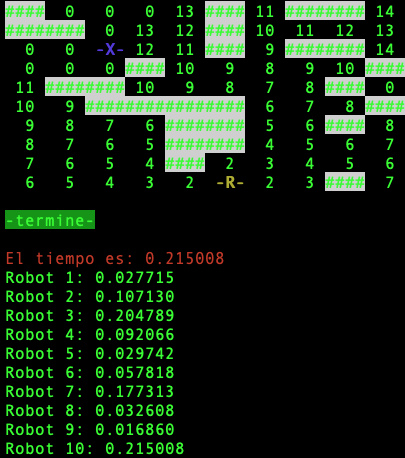
\includegraphics[scale=0.5]{image1.png}

\subsection{Plot \& table}

The larger the matrix, the longer it will take to solve the problem.

\begin{table}[!hbt]
  \caption{Problem Size vs Time}
  \centering
  \begin{tabular}{|l|l|}
    \hline
    P1 & 0.232747 \\ \hline
    P2 & 0.369061 \\ \hline
    P3 & 0.809046 \\ \hline
    P4 & 0.624046 \\ \hline
    P5 & 0.787176 \\ \hline
    P6 & 1.743657 \\ \hline
  \end{tabular}
\end{table}

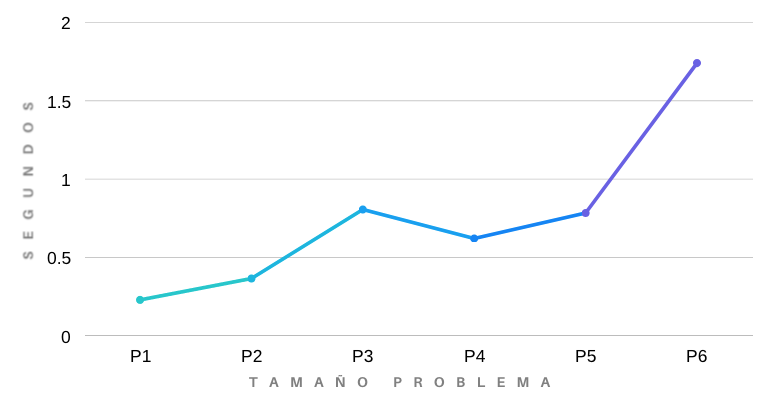
\includegraphics[scale=0.27]{plot.png}
%------------------------------------------------

\section{Conclusions}

The wavefront expansion algorithm is a technique used to parallelize the processing of graph algorithms. This algorithm works by processing vertices in a wave-like manner, where vertices in the same wavefront are processed in parallel. The wavefront expansion algorithm has been shown to be highly efficient for certain types of graphs and is commonly used in parallel programming.

It's worth noting that the actual complexity of the wavefront expansion algorithm without a queue may be influenced by the specifics of the environment and the requirements of the specific use case. For example, if the environment is sparse, with large areas of empty space, the number of iterations may be significantly reduced, which would decrease the time complexity.\\

In general, the wavefront expansion algorithm without a queue is not as efficient as the version that uses a queue, as the time complexity is higher. However, this alternative version may still be useful in certain situations, such as environments where memory is limited and a queue data structure cannot be used.

Parallel programming refers to the design and development of applications that run simultaneously on multiple processors or cores. It enables faster and more efficient processing by dividing a problem into smaller, parallelizable tasks that can be executed in parallel. The wavefront expansion algorithm is an example of a parallel programming technique that can be used to speed up the processing of graph algorithms.

%----------------------------------------------------------------------------------------
%	REFERENCE LIST
%----------------------------------------------------------------------------------------
\onecolumn
\begin{thebibliography}{99} % Bibliography - this is intentionally simple in this template
  
\bibitem[George A. Bekey, 2005]{GeorgeABekey:2005dg}
  George A. Bekey - Autonomus Robots From Biological Inspiration to Implementation and Control - MIT Press (2005).
  \newblock {\em ISBN}, 0-262-02578-7

\bibitem[Ronald C. Arkin, 1998]{RonaldCArkin:1998dg}
  Ronald C. Arkin - Behavior Based Robotics - MIT Press (1998).
  \newblock {\em ISBN}, 978-0-262-01165-5

\bibitem[Zidane,Issa and Ibrahim,Khalil, 2018]{article1:2018dg}
  Wavefront and A-Star Algorithms for Mobile Robot Path
  \newblock {\em ISBN}, 978-3-319-64860-6

\bibitem[Zhang,Han-ye and Lin,Wei-ming and Chen,Ai-xia, 2018]{article2:2018dg}
  Path Planning for the Mobile Robot: A Review
  \newblock {\em ISSN}, 2073-8994 

\bibitem[Wu,Sifan and Du,YU and Younghua Zhang, 2020]{article3:2020dg}
  Mobile Robot Path Planning Based on a Generalized Wavefront Algorithm. Mathematical Problems in Engineering Volume 2020
  \newblock {\em Article ID}, 6798798 Volume 2020

\bibitem[Bhavya Ghai and Anupam Shukla BV- Indian Institute of Information Technology and Management]{article4:2018dg}
  Wave front Method Based Path Planning Algorithm for
Mobile Robots
  \newblock {\em ISSN}, 2073-8994 

\bibitem[Ansuategui A, Arruti A, Susperregi L, Yurramendi Y, Jauregi E, Lazkano E, Sierra B., 2014]{article5:2018dg}
  Robot trajectories comparison: a statistical approach.
  \newblock {\em ScientificWorldJournal}, 2014;2014:298462

  \bibitem[Michael Soulignac, Patrick Taillibert, Michel Rueher]{article6:2008dg}
  Adapting the Wavefront Expansion in Presence of Strong Currents.
  \newblock {\em 2008 IEEE}, International Conference on Robotics and Automation
  
    
\end{thebibliography}

%----------------------------------------------------------------------------------------

\end{document}
